\documentclass[a4paper,12pt]{article}
\usepackage[a4paper, margin=1in]{geometry}
\usepackage[utf8]{inputenc}
\usepackage{graphicx}
\usepackage{xcolor}
\usepackage{braket}
\usepackage{amsmath} 
\usepackage{amssymb}
\usepackage{caption}
\usepackage[headings]{fancyhdr}
\graphicspath{ {./Figures/} }
\usepackage[sorting=none]{biblatex}
\addbibresource{refs.bib}

\usepackage{hyperref}
\hypersetup{
    colorlinks=true,
    linkcolor=black,
    urlcolor=cyan,
    citecolor=blue
}

\newcommand{\mytodo}[1]{\textcolor{red}{TODO: #1}}
\newcommand{\thetas}{\vec{\theta}}
\newcommand{\del}{\partial}
\newcommand{\base}{\mathcal{B}}
\newcommand{\e}[1]{ 10^{#1}}
\newcommand{\tvect}[2]{{#1 \choose #2}}

\DeclareMathOperator{\tr}{Tr}
\DeclareMathOperator{\Var}{Var}
\DeclareMathOperator{\tol}{tol}

\newtheorem{definition}{Definition}
\newtheorem{theorem}{Theorem}


\newenvironment{denseitemize}%
  {\begin{itemize}%
    \setlength{\itemsep}{0pt}}%
  {\end{itemize}}

% \let\OLDenumerate\enumerate
% \renewcommand\enumerate{\OLDenumerate\addtolength{\itemsep}{0.1pt}}


\title{Mutual Unbiased Bases as a Countermeasure to Barren Plateaus in Variational Quantum Algorithms}

\author{Ittay Alfassi\footnote{Email: ittay.al@cs.technion.ac.il}}

\begin{document}
\maketitle

\thispagestyle{fancy}
\fancyhead[RO]{Project Supervisor:\\{Prof. Tal Mor}}
\fancyhead[LO]{{Project in Advanced Programming - 236503}\\{Project Report}}

\tableofcontents

\section{Introduction}
Noisy, Intermediate-Scale Quantum (NISQ) computers are quantum computers that are limited in certain ways. They are usually limited in the number of qubits, connectivity between qubits, noise, and maximal circuit depth.
A computational paradigm that utilizes NISQ devices is the paradigm of hybrid quantum-classical algorithms.
Most hybrid algorithms translate a given problem into an optimization problem.
The parameters of the optimization problem control a parametrized quantum circuit, the problem's cost function is evaluated on the quantum computer, and the optimization steps are performed by the classical computer. The power of such translations is that the cost function can be efficiently calculated only on a quantum computer. These algorithms are called Variational Quantum Algorithms (VQAs)~\cite{Cerezo2021}.

While being a leading methodology for the use of quantum computers today, VQAs suffer from several problems. One such problem is the problem of Barren Plateaus~\cite{mcclean_barren_2018}. Informally, barren plateaus imply that over the optimization parameter space, the gradient of the cost function is negligibly small and the optimization process does not know how to converge.

This problem affects many  VQAs that employ different types of quantum circuits and classical optimizers (even those that are gradient-free). As the number of qubits and the depth of the quantum circuits increase, this problem worsens exponentially.
Effectively, this means that VQAs will not be able to give an advantage over their classical counterparts in problems that are not small in size.

To address this issue, in this project, I will try and utilize Mutually Unbiased Bases (MUBs), their states, and their properties.
The basic intuition behind this method is that, for any number of qubits, the set of all MUB states spans the entire Hilbert space (with real coefficients).

Thus, inserting them (in some fashion) into the optimization process can allow for an ``exhaustive search'' over the Hilbert space of all states.

Unfortunately, this method did not succeed. However, I will detail the different aspects of this approach, the experiments implemented, the conclusions I reached, and possible methods to still utilize the idea of MUB states in VQAs.

This project is mainly based on the work of Arrasmith et al.~\cite{arrasmith_effect_2021}.


\section{Preliminaries}

\subsection{Variational Quantum Algorithms}
A Variational Quantum Algorithm is an algorithm that takes some computational problem and solves it by hybrid classical-quantum optimization.
VQAs are comprised of several elements: The quantum circuit, the cost function, and the optimizer.

\begin{enumerate}
    \item \textbf{The Quantum Circuit.} Every VQA problem uses a quantum circuit with some parametric values.
    Its structure can be generally written as the following:
    \begin{equation}
        U(\thetas) = \prod_{l=1}^{L} U_l(\theta_l) W_l
    \end{equation}
    Where $U_l(\theta_l) = \exp(-i\theta_l V_l)$, $V_l$ is a Hermitian operator (thus $U_l$ is a unitary operator), and $W_l$ is a generic unitary operator that does not depend on any angle $\theta_l$.
    
    In some VQAs, an \textbf{initial state} $\ket{\psi_0}$ is also a part of the algorithm, and it is related to the quantum circuit.

    The term \emph{ansatz} (German for ``approach''/``attempt'') is used in literature to either describe the initial state $\ket{\psi_0}$, the parametric circuit $U(\thetas)$, or the application of the parametric circuit to the initial state $\ket{\psi(\thetas)} = U(\thetas)\ket{\psi_0}$.
    In this project, I will use the term ansatz to refer to the parametric quantum circuit.

    Ansatzes\footnote{The plural form of ansatz in German is Ansaetze.} can either be problem-specific or problem-agnostic.

    A problem-specific ansatz is tailored to the problem solved by the VQA using a-priori knowledge of the structure of the problem. Through this tailoring, there is a better chance that the circuit can reach values that are optimal for the problem at hand. When using a problem-specific ansatz, the initial state is usually also tailored according to the same information.
    
    A problem-agnostic ansatz is not tailored to the problem specifically and can be used with no relevant information. It is usually comprised of repeated layers of quantum gates. Each layer is comprised of quantum gates that are usually easy to implement directly on quantum hardware, in contrast to problem-specific ansatzes. Problem-agnostic ansatzes are usually called ``hardware-efficient'' for this reason.
    In this project, I focused on using hardware-efficient ansatzes.
    
    \item \textbf{The Cost Function.} The cost function $C(\thetas)$ defines the goal of the VQA. It is defined as a function from the parameters of the ansatz to the real numbers.
    The goal of the VQA is to find
    \begin{equation}
        \thetas^* = \arg\min_{\thetas} C(\thetas)
    \end{equation}

    The cost function always depends on the ansatz, some Hermitian operators, and some initial states.
    Generally, it can be written as
    \begin{equation} \label{eqn:general_cost}
        C(\thetas) = \sum_k f_k(\tr[O_k U(\thetas) \rho_k U^\dagger(\thetas)])
    \end{equation} 
    Where $\{f_k\}$ is a set of functions, $\{O_k\}$ is a set of operators, and $\{\rho_k\}$ is a set of input states.
    
    The trademark of VQAs is that they use a quantum computer to estimate the cost function $C(\thetas)$ (or its derivatives) while leveraging the power of classical optimizers to train the parameters $\thetas$.
    
    \item \textbf{The Optimizer.} While not necessarily dependent on the problem the VQA is trying to solve, the classical optimizer is an important part of the algorithm.
    The optimizer is run on a classical computer, and performs an iterative process: it uses data on the current parameters of the cost function to calculate their value in the next iteration. More details can be found in subsection~\ref{subsec:optimizers}.
\end{enumerate}


\subsubsection{Example: Variational Quantum Eigensolver} \label{subsec:vqe}
One of the earliest examples of a VQA is the VQE algorithm, proposed by Peruzzo et al.~\cite{peruzzo_variational_2014}. In this algorithm, The goal is to find the lowest eigenvalue of some Hamiltonian $H$.
The cost function is straightforwardly defined as the expectation value of the parametric state over the Hamiltonian:

\begin{equation} \label{eqn:vqe_cost}
    C(\thetas) = \bra{\psi(\thetas)} H \ket{\psi(\thetas)} = \bra{\psi_0} U^\dagger(\thetas) H U(\thetas) \ket{\psi_0}
\end{equation}

In case $H$ is a molecular Hamiltonian (converted to a qubit Hamiltonian using an appropriate transformation), a problem-specific ansatz can be used. One such option is the Unitary Coupled-Cluster (UCC) ansatz, together with the Hartree-Fock state as the initial state.

Of course, a hardware-efficient ansatz can be used for any structure of $H$.

\subsubsection{Example: Variational Quantum Compiling} \label{subsec:vqc}
A different example of a VQA is the problem of Variational Quantum Compiling (VQC), initially defined by Khatri et al.~\cite{khatri_quantum-assisted_2019} as Quantum-Assisted Quantum Compiling (QAQC).

In VQC, the input of the problem is a general $n$-qubit unitary operation $V$.\footnote{In the Khatri paper, the target unitary is denoted as $U$, while the ansatz is denoted $V$. I switched the notations to stay consistent with the rest of the examples and papers.} The goal of the algorithm is to control the parameters of a parametric quantum circuit $U(\thetas)$ so its behavior will be similar to that of $V$.

Formally, there are two possible goals: either that $U(\thetas)$ and $V$ will perform the same operation on all states, or that $U(\thetas)$ and $V$ will perform the same operation on a specific input state.
In this project, I will use the latter as the problem definition. Thus, we wish that $V\ket{\vec{0}} = U(\thetas)\ket{\vec{0}}$.

There are two different cost functions presented in~\cite{khatri_quantum-assisted_2019}.
The first is straightforward and is defined by

\begin{equation}
    C^{\textrm{global}} = 1 - \left|\bra{\vec{0}}UV^\dagger\ket{\vec{0}}\right|^2
\end{equation}

Another cost function, called the local cost function, is defined by 

\begin{equation}
    C^{\textrm{local}} = 1 - \frac{1}{n} \sum_{j=1}^{n} p_0^{(j)}
\end{equation}

where
\begin{equation} \label{eqn:local_vqc_cost}
    p_0^{(j)} = \tr[({\ket{0}\bra{0}}_j \otimes I) U^\dagger V \ket{\vec{0}}\bra{\vec{0}} V^\dagger U]
\end{equation}
and ${\ket{0}\bra{0}}_j \otimes I$ is the tensor product of the matrix $\ket{0}\bra{0}$ in the jth term and identity matrices in all other terms.
The operational meaning of $p_0^{(j)}$ is the probability to obtain the zero measurement outcome on qubit $j$ for the state $U^\dagger V\ket{\vec{0}}$.

it is proven in~\cite{sharma_noise_2020} that

\begin{equation}
    C^{\textrm{local}} \leq C^{\textrm{global}} \leq nC^{\textrm{local}}
\end{equation} 

However, $C^\textrm{global}$ suffers from a provably vanishing gradient as $n$ increases, while $C^\textrm{local}$ does not. Thus, we will use $C^\textrm{local}$ or a linear combination of both costs in our experiments.

\subsection{Optimizers for Variational Quantum Algorithms} \label{subsec:optimizers}
Classical optimizers perform the task of finding a (hopefully global) extremum of some scalar function.
An optimizer for a function $F$ needs to find the vector $\thetas \in S$ with $S \subseteq \mathbb{R}^n$ that gives a minimal or maximal value for $F$. In this project, we will only use optimizers for the minimization of cost functions.

In each step, an optimizer is given a point in the parameter space of the cost function $\thetas_{i}$, and is tasked with finding a new guess for parameter values $\thetas_{i+1}$, which hopefully has a lower cost value.

The optimizer can either use the value of the cost function, its partial derivative (its gradient vector), or its second partial derivatives (its Hessian matrix).

Methods that use the second derivative are often called Newton methods (as Newton's method uses the second derivative). Methods that use \emph{approximations} of the first and second derivative are called Quasi-Newton methods.
Methods that use the first derivative are called Gradient-Based methods. Methods that do not use the derivative at all are called Gradient-Free methods.

In this project, I focused on two gradient-free optimizers: the Powell optimizer and the COBYLA optimizer.

\subsubsection{Powell}
The Powell algorithm~\cite{Powell1964} is a popular gradient-free optimizer that uses sequential line searches (optimizations over lines in the parameter space).

This method starts with some input set of search vectors $V = \{\vec{v}_i\}$, which are usually chosen to be the coordinate vectors in the parameter space. Each vector defines a search direction (both the direction of the vector and its negation).

Searching along each of those directions in sequence, this method looks for the displacement $\{a_i\}$ along each direction that would minimize the cost when only varying parameters along the current direction.
If bounds to the parameter space are specified, the minimization will be under said bounds. If bounds are not provided, then an unbounded line search will be used.
Finding the displacements in each direction is done by some univariate gradient-free optimizer.
Two common options for such an optimizer are Brent's parabolic interpolation method and the Golden-section search method, but their choice is independent of the general Powell method.

After sweeping through all of the search vectors, two updates are made:
First, the current parameters are updated by the rule:
\begin{equation}
    \thetas_{i+1} = \thetas_{i} + \sum_i a_i \vec{v}_i
\end{equation}
Second, the search vector $\vec{v}_j$ that corresponds to the greatest displacement, $a_j = \max(a_i)$ is replaced with
\begin{equation}
    \vec{v_j} \to \sum_i a_i \vec{v}_i.
\end{equation}

The algorithm iterates an arbitrary number of times until no significant improvement to the value of the cost function is made.


\subsubsection{COBYLA}
Constrained Optimization BY Linear Approximation (COBYLA) is a gradient-free numerical optimization method, invented by Powell~\cite{Powell1994,powell_view_2007} (although it is different from the Powell optimization method).

The method tries to optimize a function $F(\thetas)$ according to a set of constraints $\{c_i(\thetas)\}$.

At each iteration, the method has $m+1$ points $\{\thetas_i\}_{i=0}^m$ in the parameter space that are sorted by a combination of the function's value on them and the penalties that the constraints imply on them.
The said sorting function is of the form
\begin{equation}
    \Phi(\thetas) = F(\thetas) + \mu[ \max\{-c_i(\thetas) : i=1,2,\dots,m \} ]_+, \thetas \in \mathbb{R}^n
\end{equation}
For a value $\mu$ that is automatically controlled by the method and the subscript + signifying that 0 is taken in case the value of the expression is negative.
Thus, our points are sorted as $\Phi(\thetas_0) < \Phi(\thetas_1) < \dots < \Phi(\thetas_m)$.

In addition, there is a ``trust region'' with a radius $\rho>0$. The method uses the $m+1$ points as the vertices of a simplex (an $m$-dimensional generalization of a triangle).
The values of the cost function in these vertices are used for interpolation to a unique linear polynomial $\hat{F}(\thetas)$, and the values of the constraint functions in these vertices are used for interpolation to unique linear constraints $\{\hat{c}_i\}$
The method then continues by minimizing $\hat{F}(\thetas)$, which is in the trust region --- that is, $\frac{\rho}{2} \leq \|\thetas - \thetas_0\| \leq \rho$, under the approximated constraints $\{\hat{c}_i\}$.

In case there is no point in the trust region in which all approximated constraints are satisfied, $\thetas$ is defined by minimizing the greatest of the constraint violations subject to the trust region bound.

The newly calculated point is added to the set of points, and some other point is removed.
The choice of the point to be removed is governed mainly by avoiding the degenerate situation where the volume of the simplex collapses to zero, as in that case, only a subspace of the parameter space is reachable.

When the improvements are insufficient, the value of $\rho$ is reduced, until some lower bound, which specifies the termination of the method, is reached.

This explanation of the method is incomplete, and only describes the general principle behind the optimization. In addition, different specifications by Powell (for example, \cite{Powell1994} and \cite{powell_view_2007}) define certain requirements and symbols differently, such as using $\Phi$ or $F$ for the sorting of vertices, the use of $\mu$, and the use of $\rho$ as the trust radius or as a lower bound for it.
Certain technical details and special steps in the method are also omitted and can be found in section 2 of~\cite{Powell1994}.


\section{Barren Plateaus} \label{sec:bps}
Informally, a barren plateau is a large section of the parameter space in which the value of the cost function $C$ is ``flat'', and has no apparent direction in which to move in order to reach a minimum point. The term was first coined by McClean et al. in~\cite{mcclean_barren_2018}.

When considering a cost function with 2 parameters, this definition coincides with its geometrical intuition. The plane defined by $\{(\theta_1, \theta_2, C(\theta_1, \theta_2)) | (\theta_1, \theta_2) \in \mathbb{R}^2\}$ will have large, flat sections, in which the ``dips'' that represent minima are not indicated by a slope around them (other than a very small neighborhood of the minimum). Such an example can be seen in Figure~\ref{fig:bp}.

\begin{figure}[h]
    \centering
    \captionsetup{justification=centering, margin=1cm}
    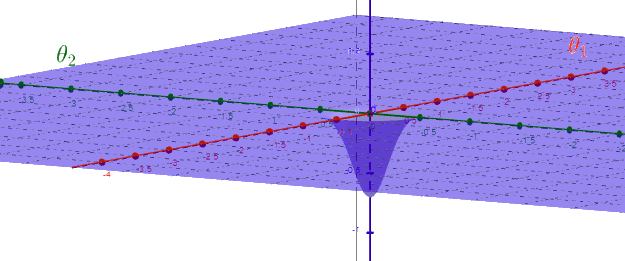
\includegraphics[scale=0.5]{bp_3d.png}
    \caption{A barren plateau in an inverted bi-variate Gaussian with a small variance.}
    \label{fig:bp}
\end{figure}

This is formally defined by the expectation value and variance of the partial derivatives.
As defined in \cite{arrasmith_effect_2021}:

\begin{definition} \label{def:bp}
    Consider the cost function defined in Eq.~(\ref{eqn:general_cost}). This cost exhibits a barren plateau if, for all $\theta_\mu \in \thetas$, the expectation value of the cost function partial derivative
    $\del C / \del\theta_\mu = \del_\mu C(\thetas)$
    is
    $E_{\thetas}[\del_\mu C(\thetas)] = 0$
    and its variance vanishes exponentially with the number of qubits n as 
    \begin{equation} \label{eqn:vanishing}
        \Var_{\thetas}[\del_\mu C(\thetas)] \leq F(n) \textrm{,   with   }F(n) \in O\left(\frac{1}{b^n}\right)
    \end{equation}
    for some $b > 1$. As indicated, the expectation values are taken over the parameters $\thetas$.
\end{definition}

\subsection{Ansatzes and Functions Affected By Barren Plateaus}
Papers in the field of barren plateaus have shown that many types of cost functions exhibit barren plateaus.

The original work by McClean et al.~\cite{mcclean_barren_2018} shows that cost functions of the form in Eq. (\ref{eqn:general_cost}) that use random quantum circuits of polynomial depth and exhibit a property known as a \emph{2-design} suffer from barren plateaus.
The definition of a 2-design is beyond the mathematical scope of this project.

However, the work of Arrasmith et al.~\cite{arrasmith_effect_2021} notes that hardware-efficient layered ansatzes are approximate 2-designs (although they did not show this result themselves).
As such, cost functions that use these ansatzes suffer from barren plateaus when the number of layers scales linearly with the number of qubits.

Another paper, by Cerezo et al.~\cite{cerezo_cost_2021}, shows that if the cost function makes use of global operators, barren plateaus will be encountered in \emph{any} circuit depth.
For this reason, it is preferable to use the local cost function in VQC problems and not the global cost function.
% A paper by Wang et al.~\cite{wang_noise-induced_2021}

\subsubsection{Barren Plateaus in VQC} \label{subsec:vqc_bp}
In section 4 of Arrasmith~\cite{arrasmith_effect_2021}, it is shown that even a fairly simple VQC problem suffers from barren plateaus.

The specific problem shown in the paper is concerned with the trivial target unitary $V = I$.
Thus, we are trying to optimize the parameters of a parametric quantum circuit $U(\thetas)$ such that $U(\thetas)\ket{\vec{0}} = I\ket{\vec{0}} = \ket{\vec{0}}$.

The quantum circuit used is a layered hardware-efficient ansatz.
Each layer is defined by the following structure:
\begin{denseitemize}
    \item A general unitary single-qubit rotation gate $U(\theta_1, \theta_2, \theta_3)$ gate is applied to each qubit.
    \item A layer of Control-NOT gates is applied between even pairs of qubits (that is, even indices act as controls and odd indices act as targets).
    \item Another layer of general unitary single-qubit rotations is applied.
    \item A layer of Control-NOT gates is applied between odd pairs of qubits (odd indices act as controls and even indices act as targets).
\end{denseitemize}
A sketch of a single layer of the circuit can be seen in Figure~\ref{fig:layer}.

The cost function used is the local VQC cost function, as shown in Eq. (\ref{eqn:local_vqc_cost}).
Arrasmith~\cite{arrasmith_effect_2021} claims that when the number of layers scales linearly with the number of qubits, this problem instance suffers from barren plateaus.

\begin{figure}[h]
    \centering
    \captionsetup{justification=centering, margin=1cm}
    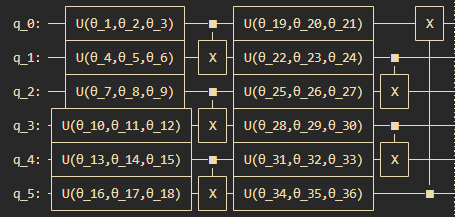
\includegraphics{arrasmith_layer.png}
    \caption{A single layer of the hardware-efficient ansatz used in the project, as designed in Qiskit.}
    \label{fig:layer}
\end{figure}

\subsection{Barren Plateaus in Gradient-Free Optimization}
Seeing as the definition of barren plateaus only discusses the partial derivatives of the cost function, one might assume that using gradient-free optimizers solves this issue.
However, the main result of Arrasmith shows that this is incorrect.

The following theorem is shown in~\cite{arrasmith_effect_2021}:

\begin{theorem}
    Consider the cost function of Eq.~(\ref{eqn:general_cost}). Let ${\thetas}_A$ and $\thetas_B$ be two randomly chosen points in parameter space.
    Without loss of generality we assume that $\thetas_B = \thetas_A + L\hat{l}$ for random $L$ and $\hat{l}$ so that $E_{\thetas_A, \thetas_B}[\dots] = E_{\thetas_A, L, \hat{l}}[\dots]$.
    If the cost exhibits a barren plateau according to Definition~\ref{def:bp}, then the expectation value of the difference $\Delta C = C(\thetas_B) - C(\thetas_A)$ is $E_{\thetas_A, L, \hat{l}}[\Delta C] = 0$, and the variance is exponentially vanishing with n as 
    \begin{equation}
        \Var_{\thetas_A,L,\hat{l}}[\Delta C] \leq \hat{G}(n)
    \end{equation}
    with
    \begin{equation}
        \hat{G}(n) = m^2 \bar{L}^2 F(n)\textrm{,    and     } \hat{G}(n) \in \tilde{O}\left(\frac{1}{b^n}\right).
    \end{equation}
    for some $b>1$. Here m is the dimension of the parameter space, $F(n)$ was defined in (\ref{eqn:vanishing}), and
    \begin{equation}
        \bar{L} = E_{L,\hat{l}}[L]
    \end{equation}
    is the average distance between any two points in parameter space.
\end{theorem}

The effective meaning of this theorem is that the difference in the cost function between different points in the parameter space is exponentially vanishing in $n$.
Thus, even though gradient-free optimizers do not use derivatives, they are still affected --- Their main tool for decision-making, which is the difference in the values of the function, gives almost no information.

\section{Mutually Unbiased Bases}
The state space of an $n$-qubit system is a $2^n$ dimensional Hilbert space.
As such, an orthonormal basis for said space contains $2^n$ distinct vectors.
There are infinitely many bases for such a space, but some combinations of bases exhibit special properties. One property, which is the main focus of this project, is \emph{Mutual Unbias}.

The following is a definition for Mutually Unbiased Bases~\cite{bandyopadhyay_new_2002}:
\begin{definition}
    Let $\base_1 = \{\ket{\phi_i}\}$ and $\base_2 = \{\ket{\psi_i}\}$ be two orthonormal bases in the $d$ dimensional state space.
    They are said to be \textbf{mutually unbiased bases (MUB)} iff the following holds:
    \begin{equation}
        \forall i,j : |\langle \psi_i | \phi_j \rangle | = \frac{1}{\sqrt{d}}
    \end{equation}
    A set $\{\base_1,\dots,\base_m\}$ of orthonormal bases in $\mathbb{C}^d$ is called a \emph{set of mutually unbiased bases} (a set of MUB) if each pair of bases $\base_i$ and $\base_j$ are mutually unbiased.
\end{definition}

The intuition for such a definition is that, if a state from one basis is measured in the other, every measurement possibility has equal probability.

In general, the term ``MUB set'' refers to a set of bases that are pairwise mutually unbiased.
The term ``MUB states'', in the context of some MUB set, is the collection of states that comprises the MUBs of that set.

\subsection{Generation of Mutually Unbiased Bases} \label{subsec:mub_gen}
The question of the existence, number, and generation of MUB sets is only answered for certain cases.

The following result has been achieved~\cite{bandyopadhyay_new_2002}:
For an $d$-dimensional state space, if $d$ is prime or a prime power ($p^k$ for a prime $p$ and a natural number $k$), there exists a set of $d+1$ MUBs.
There is constructive proof for this result.
Because the dimension of an $n$-qubit state space is $2^n$ (a prime power), there is a construction for $2^n+1$ MUBs for every $n$.

It is important to note, of course, that once a MUB set is found, there is an infinite amount of possibilities for MUB sets of the same size. Applying any arbitrary unitary $U$ to all states of the set of bases will preserve the constraints on the inner products of every pair of states, which gives a new MUB set (assuming $U$ did not act as a permutation on the set).

Connections between the problem of finding MUB sets and other problems have been made. For example, Lawrence et al.~\cite{lawrence_mutually_2002} showed that the set of $4^n-1$ Pauli operators (in the $n$-qubit case) can be partitioned into $2^n+1$ distinct subsets, each consisting of $2^n-1$ commuting operators. The same work shows two interesting conclusions:
\begin{itemize}
    \item The set of eigenbases that mutually diagonalize each subset is a set of MUBs.
    That is, if each subset $\mathcal{F}_i$ is mutually diagonalized by an orthonormal basis $\base_i$, then the set $\{\base_i\}$ is a MUB set.
    \item Each such partitioning defined a unique choice of $2^n+1$ MUBs in the $n$-qubit Hilbert space.
\end{itemize}

I used the examples given in the work of Lawrence et al. to construct a set of MUBs for 2 and 3 qubits.
However, it is important to note that the generation of MUBs in this fashion requires exponential time in the number of qubits: it requires the simultaneous diagonalization of matrices that are exponential in size.

\subsection{MUB States as an Exhaustive Search}

The set of MUB states for one qubit is well known. The set contains 3 MUBs, and each basis is the eigenbasis of a Pauli matrix.
Specifically, the bases and states are
$$ \base_z = \{ \ket{0}, \ket{1}\}  = \{\tvect{1}{0}, \tvect{0}{1}\}$$
$$ \base_x = \{ \ket{+}, \ket{-}\}  = \{\frac{1}{\sqrt{2}}\tvect{1}{1}, \frac{1}{\sqrt{2}}\tvect{1}{-1}\}$$
$$ \base_y = \{ \ket{+_i}, \ket{-_i}\}  = \{\frac{1}{\sqrt{2}}\tvect{1}{i}, \frac{1}{\sqrt{2}}\tvect{1}{-i}\}$$

When displayed on the Bloch sphere, these states are presented as the poles of the sphere in the z, x, and y axes, appropriately. As such, every 1-qubit state is reachable through a linear combination of these six states with real coefficients.

This is our initial intuition: these states reach every pole of the sphere that defines all 1-qubit states.
We (Tal Mor and I) believed that this can be extended to higher dimensions. If our hypothesis of the importance of MUBs is correct, they can be useful when trying to check for a certain property, \textbf{or when searching for a specific point in space.}

An observation made in~\cite{lawrence_mutually_2002} supports our hypothesis.
In~\cite{lawrence_mutually_2002}, a MUB is generated by being the orthonormal basis that mutually diagonalizes a subset of Pauli operators.
Let $\{O_i\}$ be such a subset of Pauli operators, and let $\{\ket{\psi_i}\}$ be the mutually diagonalizing eigenbasis calculated for that subset.
Let $U_i(\theta) = exp(-i\theta O_i)$ be a unitary high-dimensional rotation defined by $O_i$.
When $U_i$ acts on a MUB state $\ket{\psi_j}$, that state is not affected (up to a global phase) \textbf{and acts as a pole}.

In the next section, I will discuss the different methods to use the concept of MUB states as an exhaustive search in mitigating barren plateaus.


\section{MUB Utilization Techniques} \label{sec:mub_use}
This section specifies the novel ideas that Tal and I had for the project. As such, they are comprised of theoretic extensions and assumptions that we made.

To explain our idea, let us consider a VQA in which the target is to reach a specific state.
One such example is VQE (section~\ref{subsec:vqe}), in which the lowest eigenvalue is calculated by reaching the lowest eigenstate.
An example of utilizing MUBs in a different type of VQA is given in subsection~\ref{subsec:mub_vqc}.

Let us make the following assumptions:
\begin{enumerate}
    \item The cost function $C(\thetas)$ (shown in Eq.~(\ref{eqn:vqe_cost})) experiences a barren plateau in the parameter space. 
    \item The optimization starts with a specific initial parameter vector, $\thetas_0$, whose entries were chosen uniformly randomly from the parameter space.
    \item The ansatz $U(\theta)$ is \emph{expressive} --- Every state $\ket{\psi}$ in the state has a parameter vector $\thetas_\psi$ such that $U(\thetas_\psi)\ket{\vec{0}} = \ket{\psi}$.
    \label{itm:expressive}
\end{enumerate}

The target state $\ket{\psi^*}$ that the VQA is trying to reach, according to assumption~\ref{itm:expressive}, has an appropriate parameter choice $\thetas^*$.
However, since $C(\thetas)$ suffers from barren plateaus, any optimizer cannot travel long distances in the parameter space.
Thus, if $U(\thetas_0)\ket{\vec{0}}$ is far from $\ket{\psi^*}$ (in terms of the state space), the VQA will not reach the required parameters.

However, because the MUB states act as an exhaustive search over the Hilbert space (or so we hope), there exists some MUB state $\ket{\alpha}$ such that $U(\thetas_0)\ket{\alpha}$ and $\ket{\psi^*}$ are close (in terms of the state space).
Equivalently, there exists some parameter vector $\thetas_0^\alpha$ such that $U(\thetas_0) \ket{\alpha} = U(\thetas_0^\alpha) \ket{\vec{0}}$, and $\thetas_0^\alpha$ and $\thetas^*$ are close \textbf{in terms of the parameter space}. Thus, an optimizer will be able to find an appropriate parameter set and reach $\ket{\psi^*}$ despite the barren plateaus of the cost function.

\paragraph*{Non-Uniformity of Parameter Space}~\\
An ansatz, even if fully expressive, does not necessarily bring its input to all output states in the Hilbert space with equal probability. For example, it could be that the vast majority of parameter vectors bring the result to a very small distance from the input vector.
For this reason, the use of a MUB state to dramatically shift the output result is valuable.
This phenomenon is connected to the mathematical term called \emph{Concentration of Measure} and to the Haar Measure for unitaries and states, as mentioned in~\cite{mcclean_barren_2018}.
However, the research of these terms and phenomena were left outside the scope of this report.

\paragraph*{Non-Expressive Ansatzes}~\\
While assumption~\ref{itm:expressive} seems useful (both for applications and for our analysis), it is unfortunately unrealistic.
Seeing as a general $2^n \times 2^n$ unitary matrix has an exponential number of degrees of freedom, reaching the entire set of unitary transformations requires an exponential number of parameters and an ansatz of exponential size.

Thus, the output of a hardware-efficient ansatz of linear depth will only span a small subset of the Hilbert space.
If our target is a state $\ket{\psi^*}$, it could lie outside the subset $\{U(\thetas)\ket{\vec{0}} | \thetas \in \mathbb{R}^m\}$. Using a MUB state as the input instead of $\ket{\vec{0}}$ could dramatically shift the subset and change it to include $\ket{\psi^*}$.

\medskip
The question that remains is how \emph{exactly} to use the set of MUB states.

\subsection{Using All MUB states} \label{meth:all_mub}
The most trivial idea is to attempt optimization from all possible MUB states.
That is, set a specific random initial parameter vector $\thetas_0$, and run a separate experiment with every MUB state as the initial state.

However, there is a major drawback to this method.
For $n$ qubits, there are $2^n+1$ different MUBs, with $2^n$ states each.
Thus, this requires performing $O(4^n)$ experiments for every instance of the problem, which is non-scalable for reasonable problem sizes.

\subsection{Sampling $k$ MUB states} \label{meth:k_mub}
A way to mitigate the drawback I just mentioned is to randomly sample a small number of MUB states from the entire set and only run experiments from them.

This will allow an arbitrary amount of experiments, which we can control.
In addition, as will be discussed in section~\ref{meth:random_thetas}, this serves as an interesting benchmark to compare against na{\"i}ve methods.

However, as mentioned in subsection~\ref{subsec:mub_gen}, the cost of calculation of the MUBs and their states is still exponential in time. Although the work of MUB calculation only needs to happen once and can be considered pre-processing, this makes the current suggestion unfeasible, for example, for $n>60$ qubits.

In addition, although the work of~\cite{bandyopadhyay_new_2002} shows a theoretical construction for the MUB sets for $n$ qubits, it is difficult to implement in practice.
Thus, Tal and I faced an interesting question: what can be done, for $n$ qubits, with only the MUB states for 2 and 3 qubits?

\subsection{``Half-MUB'' states} \label{meth:half_mub}
We came up with a relatively simple idea: given an $n$-qubit register, pick 2 or 3 qubits. Generate a MUB state between the chosen qubits, and keep the rest in the 0 state.

The amount of such states for $n$ qubits is polynomial. There are ${n \choose 3} = O(n^3)$ triplets for the qubit choices, and each one has a constant amount of MUB state options.
Thus, their generation (and even exhaustive experimentation with them) takes reasonable time.

This method got the nickname ``Half-MUBs'', as its results resemble MUB states but do not give the same exhaustive properties.
However, no one guaranteed that MUB states act as an exhaustive search themselves, so what the hell.

\subsection{MUB Utilization in VQC} \label{subsec:mub_vqc}
As explained in subsection~\ref{subsec:vqc}, the goal of VQC is to make the ansatz act like a specific target unitary (either in general or on a specific state).
In this sense, it deviates from the previous discussions in this section, as it does not aim to reach a specific state, but a specific transformation.
However, the claims presented in this section still apply in the case of VQC.

The only difference is that instead of considering the state Hilbert space, we look at the group of unitary transformations on $n$ qubits $U(2^n)$.
Non-Uniformity still applies: a uniform choice of parameter values for the ansatz does not necessarily send the resulting unitary to a uniformly random unitary in $U(2^n)$.
Because of that, the prepending of the MUB generation circuit to the ansatz could move it dramatically closer to the target unitary (in terms of the parameter space).
Non-expressivity applies in a similar fashion.

\section{Experiments} \label{sec:experiments}
In this section, I will detail the experiments that I implemented in the project.

Section~\ref{meth:random_thetas} explains the control group to which I compare each idea.

Section~\ref{subsec:hyperparams} details the hyper-parameters of the experiments.

Section~\ref{subsec:exp_hyperparams} details the experiments used for choosing hyper-parameters.

Section~\ref{subsec:reproduce} shows a reproduction of the barren plateau simulation presented in \cite{arrasmith_effect_2021}.

Section~\ref{subsec:mub_synthesis} details the synthesis of MUB-generating circuits.

Section~\ref{subsec:3qubits} shows experiments on 3 qubits and $k$ random MUB states.

Section~\ref{subsec:nqubits} shows experiments on higher numbers of qubits and $k$ half-MUB states.

All experiments were implemented in Python, and can be found on GitHub under the link \url{https://github.com/ittay-alfassi/barren-plateaus}.
The repository in the link contains the code for the experiments and their analysis, raw data generated by the experiments, convergence graphs for every experiment, and intermediate documents for future ideas.
Throughout the section, references to specific folders and sections in the code will be given for each experiment and its results.

MUB circuit synthesis was done using the Qsymm~\cite{qsymm} and BQSkit~\cite{bqskit} packages.
The construction and execution of quantum circuits was done using the Qiskit~\cite{qiskit} package.
The optimizers were taken from the SciPy~\cite{scipy} package.

\subsection{Control Group: Random Initialization Vectors} \label{meth:random_thetas}
A critical step that we must take before testing the use of MUBs is a na{\"i}ve equivalent.
A reasonable equivalent to using $k$ different MUB (or half-MUB) states and a single initial vector is to run $k$ experiments with no MUB states involved --- just \textbf{use a different random initial vector for each experiment}.

Note that if our ansatz is expressive (assumption \ref{itm:expressive} in section \ref{sec:mub_use}), another interesting comparison can be made.

As shown in section~\ref{sec:mub_use}, if an ansatz is expressive, every MUB state $\ket{\alpha}$ can be described as $U(\thetas^\alpha)\ket{\vec{0}}$ for some parameter vector $\thetas^\alpha$.
Thus, the comparison between $k$ MUB states and $k$ random initial vectors can be seen as a comparison between a carefully chosen set of starting parameters $\{\thetas^{\alpha} | \ket{\alpha} \textrm{ is a MUB state}\}$ and a random set of starting parameters $\{\thetas_0^i | \forall i, \thetas_{0}^{i} \in [-\pi, \pi)^m\}$.

\subsection{Experiment Hyper-Parameters} \label{subsec:hyperparams}
Every VQA experiment has, besides of the initial state and the given problem, other parameters that affect its execution.
These parameters are often called hyper-parameters (to separate them from the parameter vector of the ansatz and optimizer).
These hyper-parameters can have a deep impact on the result of the experiment.
Thus, it is important to list them and explain the choice of every hyper-parameter.

I will now list the hyper-parameters and their chosen values.
The experiments I used to choose these values are detailed in the next subsection.

\paragraph*{Optimizer}
The same optimization problem can be solved by different optimizers.
The optimizers that I used in my experiments are the gradient-free optimizers COBYLA and Powell.

\paragraph*{Tolerance Condition}
Every optimizer has certain halting conditions.
For example, an upper bound on the number of optimization iterations can be defined.
To allow for long optimization times, I did not place a max-iteration limit.

Another halting condition is the tolerance condition, often nicknamed ``tol''.
It is a condition that defines a minimal tolerance for differences in the optimization.
For example, an optimizer can require a minimum difference between two different iterations' cost values.
In general, a tolerance condition is defined as a floating point number.
For the COBYLA optimizer, the tol value is a lower bound on the size of the trust region.
For the Powell optimizer, the tol value becomes (in the words of the SciPy documentation) ``the relative error in the solution and its function value acceptable for convergence.'' The documentation gives no further details on the meaning of ``relative error''.
For the Nelder-Mead optimizer, the tol value has the same definition as the Powell optimizer.
The evidence that this is the meaning of the tol value for each optimizer was taken directly from the source code and in-code documentation of SciPy.
It can be found in the following link: \url{https://github.com/scipy/scipy/blob/main/scipy/optimize/_minimize.py}. The tolerances assignment can be found around line 600.\footnote{Who said Reverse Engineering isn't important for quantum scientists? :)}

I chose 4 different values to experiment with: $2 \times \e{-1}$, $\e{-2}$, $\e{-5}$, and $\e{-12}$. They are used in different settings, as specified in the rest of the section.

\paragraph*{Success Bound}
Another possible halting condition for an optimizer is a manual limit for the cost function's value.
For example, in the numerical simulations of Arrasmith~\cite{arrasmith_effect_2021}, they stopped the optimization process once the cost function's value reached $C=0.4$.
I call these values ``success bounds'', as they present a lower bound for the function's value, such that reaching it (or below it) counts as a success of the optimization procedure. Specifically, it signifies that we succeeded in overcoming the barren plateaus.

In my experiments, I define two different success bounds: 0.4 and 0.1.
Both are used in different settings, as specified in the rest of the section.

\paragraph*{Number of Repetitions}
Every experiment must be repeated several times to ensure the statistical significance of the results. In our case, the value $k$ (the number of MUB states, Half-MUB states, or random vectors) fits this role well.
Performing five experiments with $k=5$ in each one, then generating statistics for the collection of results is equivalent to performing a single experiment with $k=25$.
I chose to use $k=25$ in all of my experiments.

\subsection{Perliminary Experiments: Setting Hyper-Parameters} \label{subsec:exp_hyperparams}

\paragraph*{Choosing the Tolerance Condition}~\\
In SciPy, the tolerance condition of all optimizers is defined by a single floating-point parameter named ``tol''. However, its practical meaning is different for every optimizer, as specified in the previous subsection.

In order to see what tol values are appropriate for every optimizer, I tried each optimizer with four different tol values.
The task was the same: Solve the trivial VQC example with 3 qubits, 12 layers of the hardware-efficient ansatz, and a success bound of 0.1.

\paragraph*{Results.}
The results are summarized in Table \ref{tbl:tol_results}.

\begin{table}[] 
    \centering
    \begin{tabular}{|c|c|c|c|}
        \hline
        tol & COBYLA & Powell & Nelder-Mead \\ \hline
        $2 \times 10^{-1}$ & \begin{tabular}[c]{@{}c@{}}25/25 success\\ avg nfev 137.92\end{tabular} & \begin{tabular}[c]{@{}c@{}}25/25 success\\ avg nfev 211.36\end{tabular} & \begin{tabular}[c]{@{}c@{}}0/25 success\\ avg nfev 217\end{tabular} \\ \hline
        $10^{-2}$ & \begin{tabular}[c]{@{}c@{}}25/25 success\\ avg nfev 129.88\end{tabular} & \begin{tabular}[c]{@{}c@{}}25/25 success\\ avg nfev 295.52\end{tabular} & \begin{tabular}[c]{@{}c@{}}25/25 success\\ avg nfev 4302.32\end{tabular} \\ \hline
        $10^{-5}$ & \begin{tabular}[c]{@{}c@{}}25/25 success\\ avg nfev 139.6\end{tabular} & \begin{tabular}[c]{@{}c@{}}25/25 success\\ avg nfev 623.84\end{tabular} & N/A \\ \hline
        $10^{-12}$ & \begin{tabular}[c]{@{}c@{}}25/25 success\\ avg nfev 131.24\end{tabular} & \begin{tabular}[c]{@{}c@{}}25/25 success\\ avg nfev 928.64\end{tabular} & N/A \\ \hline
    \end{tabular}
    \caption{The number of successful experiments and average Number of Function EVals (nfev) for different optimizers and tol values.}
    \label{tbl:tol_results}
\end{table}
COBYLA acted similarly for all tested tolerance values.
I also tested the special case of $\tol=0$ for COBYLA. It caused an interesting bug. Because no lower bound was specified for the error, the COBYLA optimization process crashed by inputting $\infty$ and $-\infty$ into the parameter vector (seemingly at random).

Powell showed reasonable scaling for all tested tolerance values.

Nelder-Mead managed to terminate with $\tol=2 \times \e{-1}$ but failed to reach the correct solutions.
With $\tol=\e{-2}$, Nelder-Mead took approximately 20 times longer than with the previous value.
With $\tol=\e{-5}$, Nelder-Mead took over 1 hour and could not finish a single experiment. For comparison, a COBYLA run took around 20 seconds.
For this reason, I did not test with $\e{-12}$ either.

My conclusion is that COBYLA and Powell are usable with any tol value, but Nelder-Mead is only usable (and barely so) with $\tol=\e{-2}$.
Thus, the value that I chose for tol is $\e{-5}$. This value that is low enough to not stop convergence in extreme situations, but probably not so low as to waste time on fruitless runs.
The code for the experiments in this paragraph can be found under the section ``Hyper-Parameter Experiments: Choosing TOL'' in the notebook ``bps.ipynb''.
% The result data can be found under ``VQC results/tol\_experiments.txt''.

\paragraph*{Choosing the right optimizer}~\\
After choosing reasonable tol values from the results of the previous experiment, I tested the three possible optimizers (COBYLA, Powell and Nelder-Mead) with the same VQC problem, with a changing number of qubits:
From 4 qubits and 4 layers to 7 qubits and 7 layers.

\paragraph*{Results.}
The success percentages of the optimizers, both for $C=0.4$ and for $C=0.1$ are summarized in Table\mytodo{Add table.}. The average nfevs of the optimizers are shown in Figure \mytodo{Add figure!}.

\mytodo{Modify the details according to the actual results.}
Both COBYLA and Powell managed to perform well on 4-7 qubits.
Nelder-Mead took more time to finish 4 qubits than all the COBYLA experiments. Thus, it was neglected for the rest of the experiments.

Between COBYLA and Powell, COBYLA took less time to finish the optimization in most cases. Thus, I chose to use COBYLA for the rest of the experiments.
The code for the experiments in this paragraph can be found under the section ``Hyper-Parameter Experiments: Choosing the Optimizer'' in the notebook ``bps.ipynb''.

\subsection{Experiment Set 1: Reproducing the Arrasmith Barren Plateau} \label{subsec:reproduce}
In section 4 (Numerical Simulations) of Arrasmith~\cite{arrasmith_effect_2021}, a numerical demonstration of the barren plateaus in the VQC problem.
In that section, the trivial VQC problem mentioned in section~\ref{subsec:vqc_bp} is tested for $n=5,\dots,11$ qubits.
The hyper-parameters were defined as the following:
\begin{denseitemize}
    \item \textbf{Optimizer.} Four different optimizers were tested: Nelder-Mead, Powell, COBYLA, and Gradient Descent (for reference).
    \item \textbf{Success bound.} The success bound was defined as a cost value of $C=0.4$.
    \item \textbf{Number of repetitions.} Each experiment was performed $k=20$ times.
\end{denseitemize}
The tolerance condition was not specified.\\

In my recreation, I used the following parameters:

\begin{denseitemize}
    \item \textbf{Number of qubits.} I used $n=4$ to $n=9$ qubits.
    \item \textbf{Number of layers.} I used linear scaling of layers --- $n$ layers with $n$ qubits.
    \item \textbf{Optimizer.} As discussed, I used the COBYLA optimizer.
    \item \textbf{Tolerance condition.} As discussed, I used $\tol=\e{-5}$.
    \item \textbf{Success bound.} I used a terminating success bound of $0.1$, with another line specifying the cost value of $0.4$, as an additional point for comparison.
    \item \textbf{$k$.} I used $k=25$ repetitions for each method.
\end{denseitemize}

\paragraph*{Results.}
The graph of the average nfev as a function of the number of qubits is given in figure \mytodo{Add a figure!}, with an exponential scale.
The success rates of each number of qubits is given in table \mytodo{Add a table!}.

Thus, in the values that we were able to calculate, we can see that an exponential barren plateau appears, partially recreating the graph in Section 4 of Arrasmith~\cite{arrasmith_effect_2021}.

The code for the experiments in this subsection can be found in the section ``Experiment Set \#1: Barren Plateau Reproduction'' in the notebook ``bps.ipynb''.
Convergence graphs for each one of the experiments can be found in the ``VQC results/local cost barren plateaus'' subfolder. A text file with statistics and all evaluations can be found in the same folder, and used for the generation of future statistics. Details on the structure of the text file can be found in the appendix.

\subsection{Synthesis of MUBs in Code} \label{subsec:mub_synthesis}
The process of calculating the sets of MUBs for 2 and 3 qubits was straightforward.
The first step was to copy the rows of the tables in figures 2 and 3 of \cite{lawrence_mutually_2002} into the code.
Recall that each row defined a MUB: the MUB is the eigenbasis of the Pauli strings in that row.
However, the paper notes that ``particular subsets of three determine the corresponding basis sets completely''.
Thus, in the 3-qubit case, I only copied the strings from the first three columns of the table to the code.

After that, I used the Qiskit module to write out each Pauli String as a matrix and used the Qsymm module to simultaneously diagonalize the rows of matrices.

At this point, The code has generated the state vectors that correspond to each MUB state. However, we wish to generate them through a circuit.
Note that If we treat the collection of state vectors in a MUB as a matrix, we get a unitary matrix with the following property:
If we apply the matrix to a computational state $\ket{i}$, we get the i'th state of the MUB as the output.
If we synthesize a circuit that implements this unitary, we can use it to generate every MUB state from the specific MUB.

Thus, for each MUB, I used the BQSkit module to synthesize a circuit that corresponds to the MUB's unitary matrix.
The synthesized results are written in OpenQASM 2.0.
These circuits are saved as qasm files in a folder, to be used in the following experiments.

The code for the MUB circuit synthesis is in the notebook ``mub\_generation.ipynb''.
The MUB circuits can be found under the folder ``mub\_bqskit''.
The circuits for two qubits are under the subfolder ``2\_302''. The circuits for three qubits are under the subfolder ``3\_306''.


\subsection{Experiment Set 2: 3 qubits and $n$ layers} \label{subsec:3qubits}
The following experiment is the first example of a practical comparison between MUB-based experiments and non-MUB based experiments.

Parameters and hyper-parameters were defined as the following:
\begin{denseitemize}
    \item \textbf{Utilization Method.} I am using the method of ``Sampling $k$ MUB states'', described in section~\ref{meth:k_mub}. It is compared to the control group of random initial vectors from section~\ref{meth:random_thetas}.
    \item \textbf{Number of qubits.} I used $n=3$ qubits.
    \item \textbf{Number of layers.} I used 12 layers of the hardware-efficient ansatz.
    \item \textbf{Optimizer.} As discussed, I used the COBYLA and POWELL optimizers.
    \item \textbf{Tolerance condition.} As discussed, I used $\e{-5}$.
    \item \textbf{Success bound.} I used a terminating success bound of $0.1$, with another line specifying the cost value of $0.4$, as an additional point for comparison.
    \item \textbf{$k$.} I used $k=25$ repetitions for each method.
\end{denseitemize}

\paragraph*{Results.}
% The results are presented in Figures \ref{fig:3qubits_cobyla} and \ref{fig:3qubits_powell}.
The results are presented in Figure \ref{fig:3qubits_cobyla}.
\begin{figure}[]
    \centering
    \captionsetup{justification=centering, margin=1cm}
    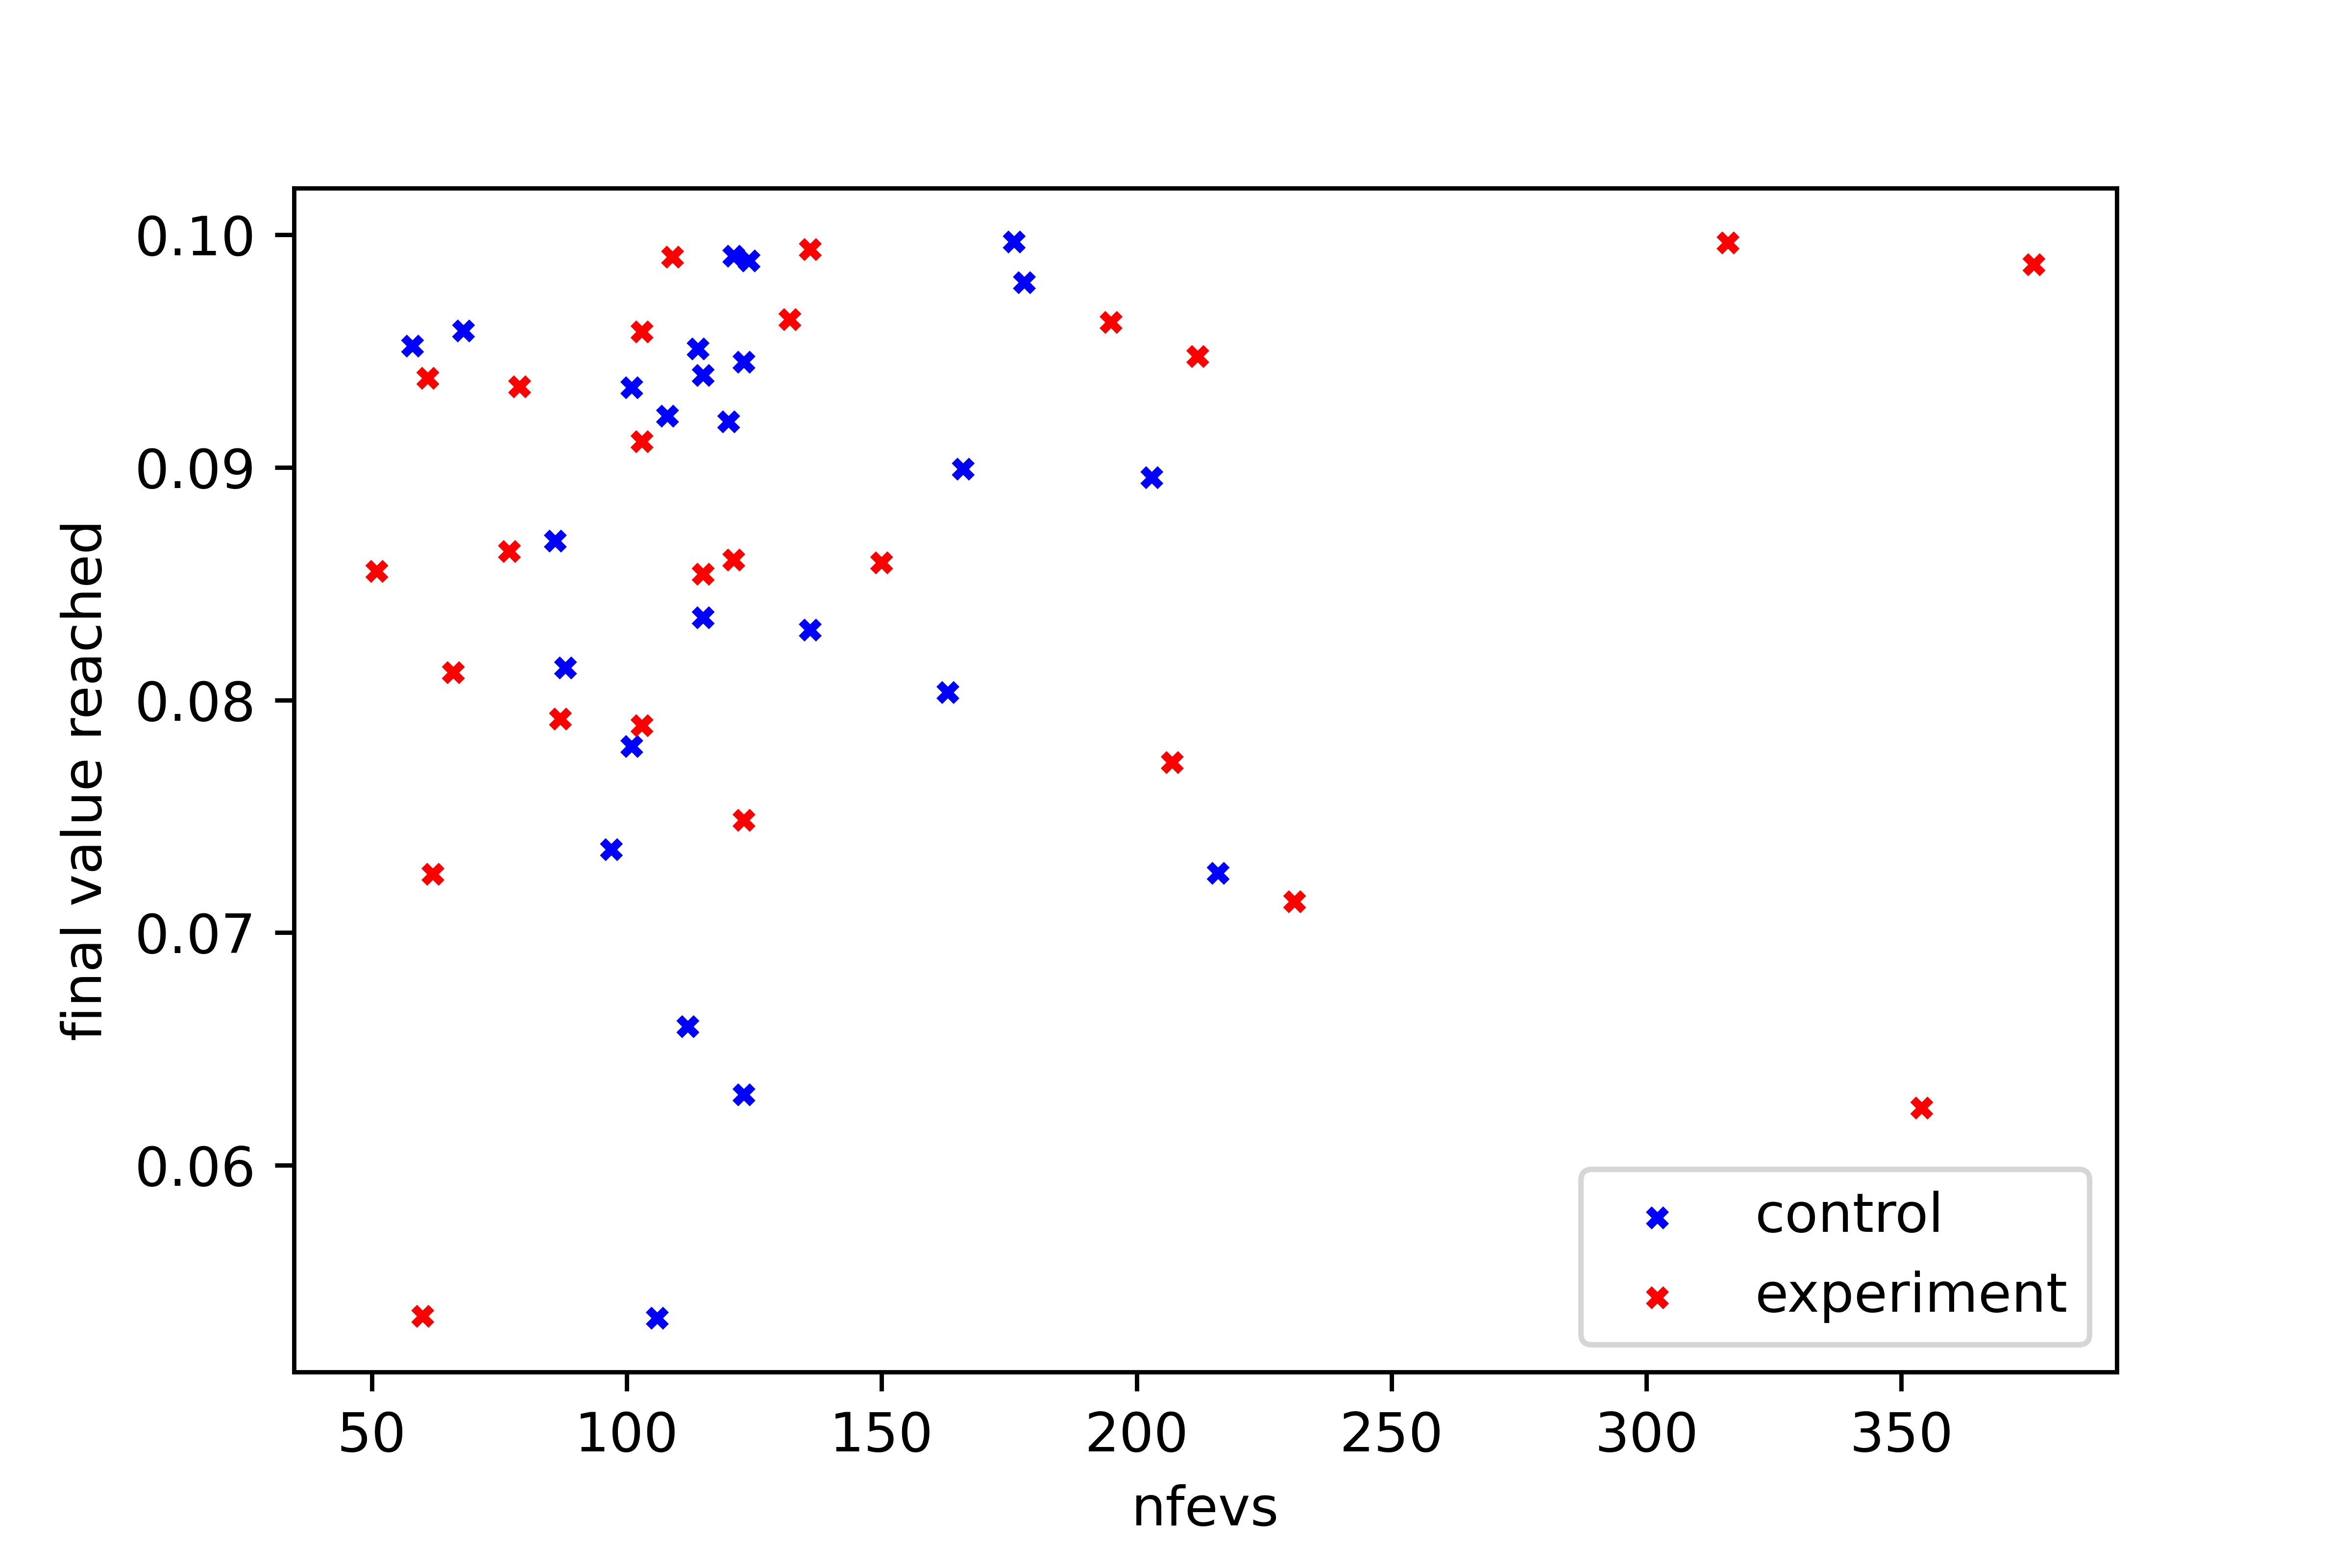
\includegraphics[scale=0.8]{3qubits_cobyla.png}
    \caption{A scatter plot of the results of Experiment 2 using COBYLA. The x-axis shows the nfevs of each experiment, and the y-axis shows the value at which the optimization halted.}
    \label{fig:3qubits_cobyla}
\end{figure}

% \begin{figure}[]
%     \centering
%     \captionsetup{justification=centering, margin=1cm}
%     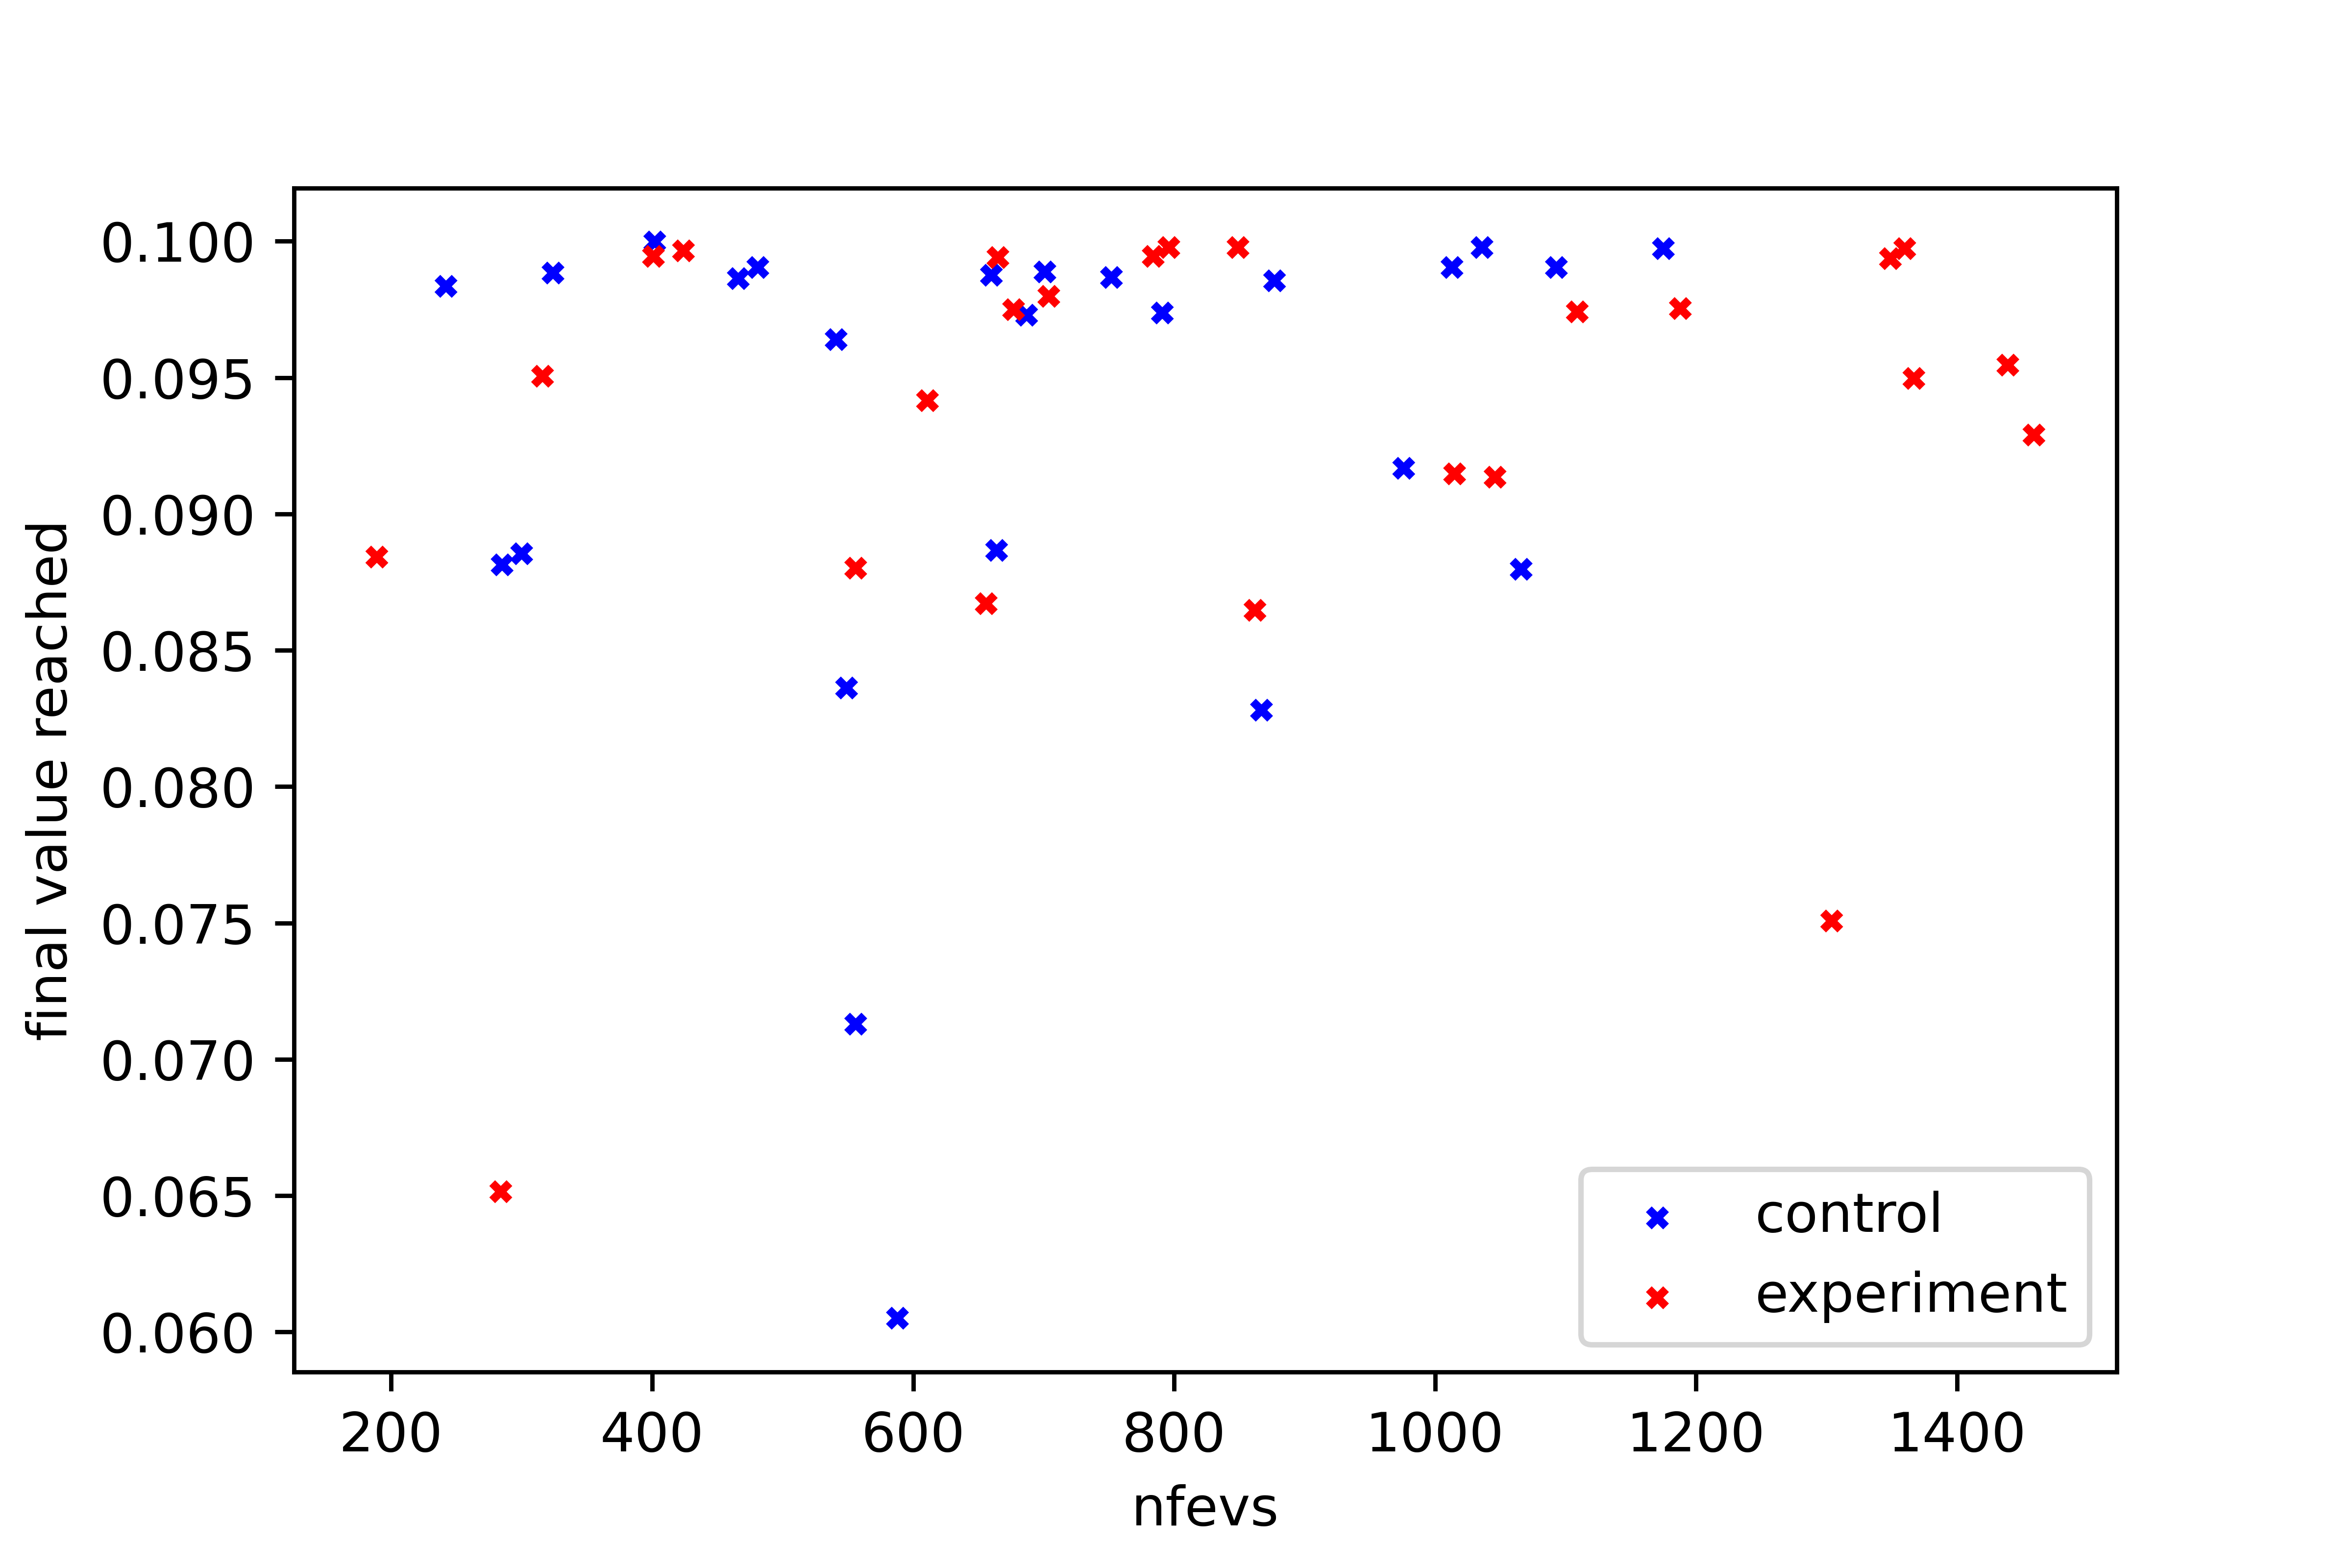
\includegraphics[scale=0.8]{3qubits_powell.png}
%     \caption{A scatter plot of the same experiment set with the Powell optimizer.}
%     \label{fig:3qubits_powell}
% \end{figure}

As shown in the scatter plot, the control group and the MUB-based experiments behaved similarly, with no clear advantage.
All runs (Control Group and MUB-based) managed to reach the $C=0.1$ success bound\footnote{Experiments that finished below the 0.1 cost value reached it in one iteration. That is, the before-last evaluation had a value above 0.1, and the last iteration had the value that is shown in the plot}.
The average nfev of the Control Group was 124.72.
The average nfev of the MUB-based experiments was 145.16.
In addition, the lowest and highest nfev counts are similar in both cases.

Thus, my conclusion is that with 3 qubits, there is no advantage to using MUB states as initial states over random initial parameter vectors.

The code for the experiments in this subsection can be found in the section ``Experiment Set \#2: 3 qubits, 12 layers'' in the notebook ``bps.ipynb''.
Convergence graphs for each one of the experiments can be found in the ``VQC results/local cost 3 qubits'' subfolder. A text file with statistics and all evaluations can be found in the same folder, and used for the generation of future statistics. Details on the structure of the text file can be found in the appendix.



\subsection{Experiment Set 3: $n$ qubits and $n$ layers} \label{subsec:nqubits}
As the last experiment showed no promise from the use of MUBs in 3 qubits, the next reasonable idea to explore is a higher number of qubits.

Parameters and hyper-parameters were defined as the following:
\begin{denseitemize}
    \item \textbf{Utilization Method.} I am using the method of ``Sampling Half-MUB states'', using 3-qubit MUB sets, described in section~\ref{meth:half_mub}. It is compared to the control group of random initial vectors from section~\ref{meth:random_thetas}.
    \item \textbf{Number of qubits.} As I showed in the optimizer hyper-parameter experiment in \ref{subsec:exp_hyperparams}, experiments started taking a considerable amount of time when the number of qubits reached 7.
    Thus, I chose to perform the high-qubit-number experiments with $n=7$ qubits.
    \item \textbf{Number of layers.} I used 7 layers of the hardware-efficient ansatz. The reason is twofold: The barren plateaus appear with linear scaling of layers with the number of qubits, and the number of parameters stays similar to experiment 2.
    3 qubits $\times$ 12 layers = 48 $\approx$ 49 = 7 qubits $\times$ 7 layers.
    \item \textbf{Optimizer.} As discussed, I used the COBYLA optimizer.
    \item \textbf{Tolerance condition.} As discussed, I used $\e{-5}$.
    \item \textbf{Success bound.} I used a terminating success bound of $0.1$, with another line specifying the cost value of $0.4$, as an additional point for comparison.
    \item \textbf{$k$.} I used $k=25$ repetitions for each method.
\end{denseitemize}

\paragraph*{Results.}
The results are presented in Figure~\ref{fig:7qubits}.

\begin{figure}[]
    \centering
    \captionsetup{justification=centering, margin=1cm}
    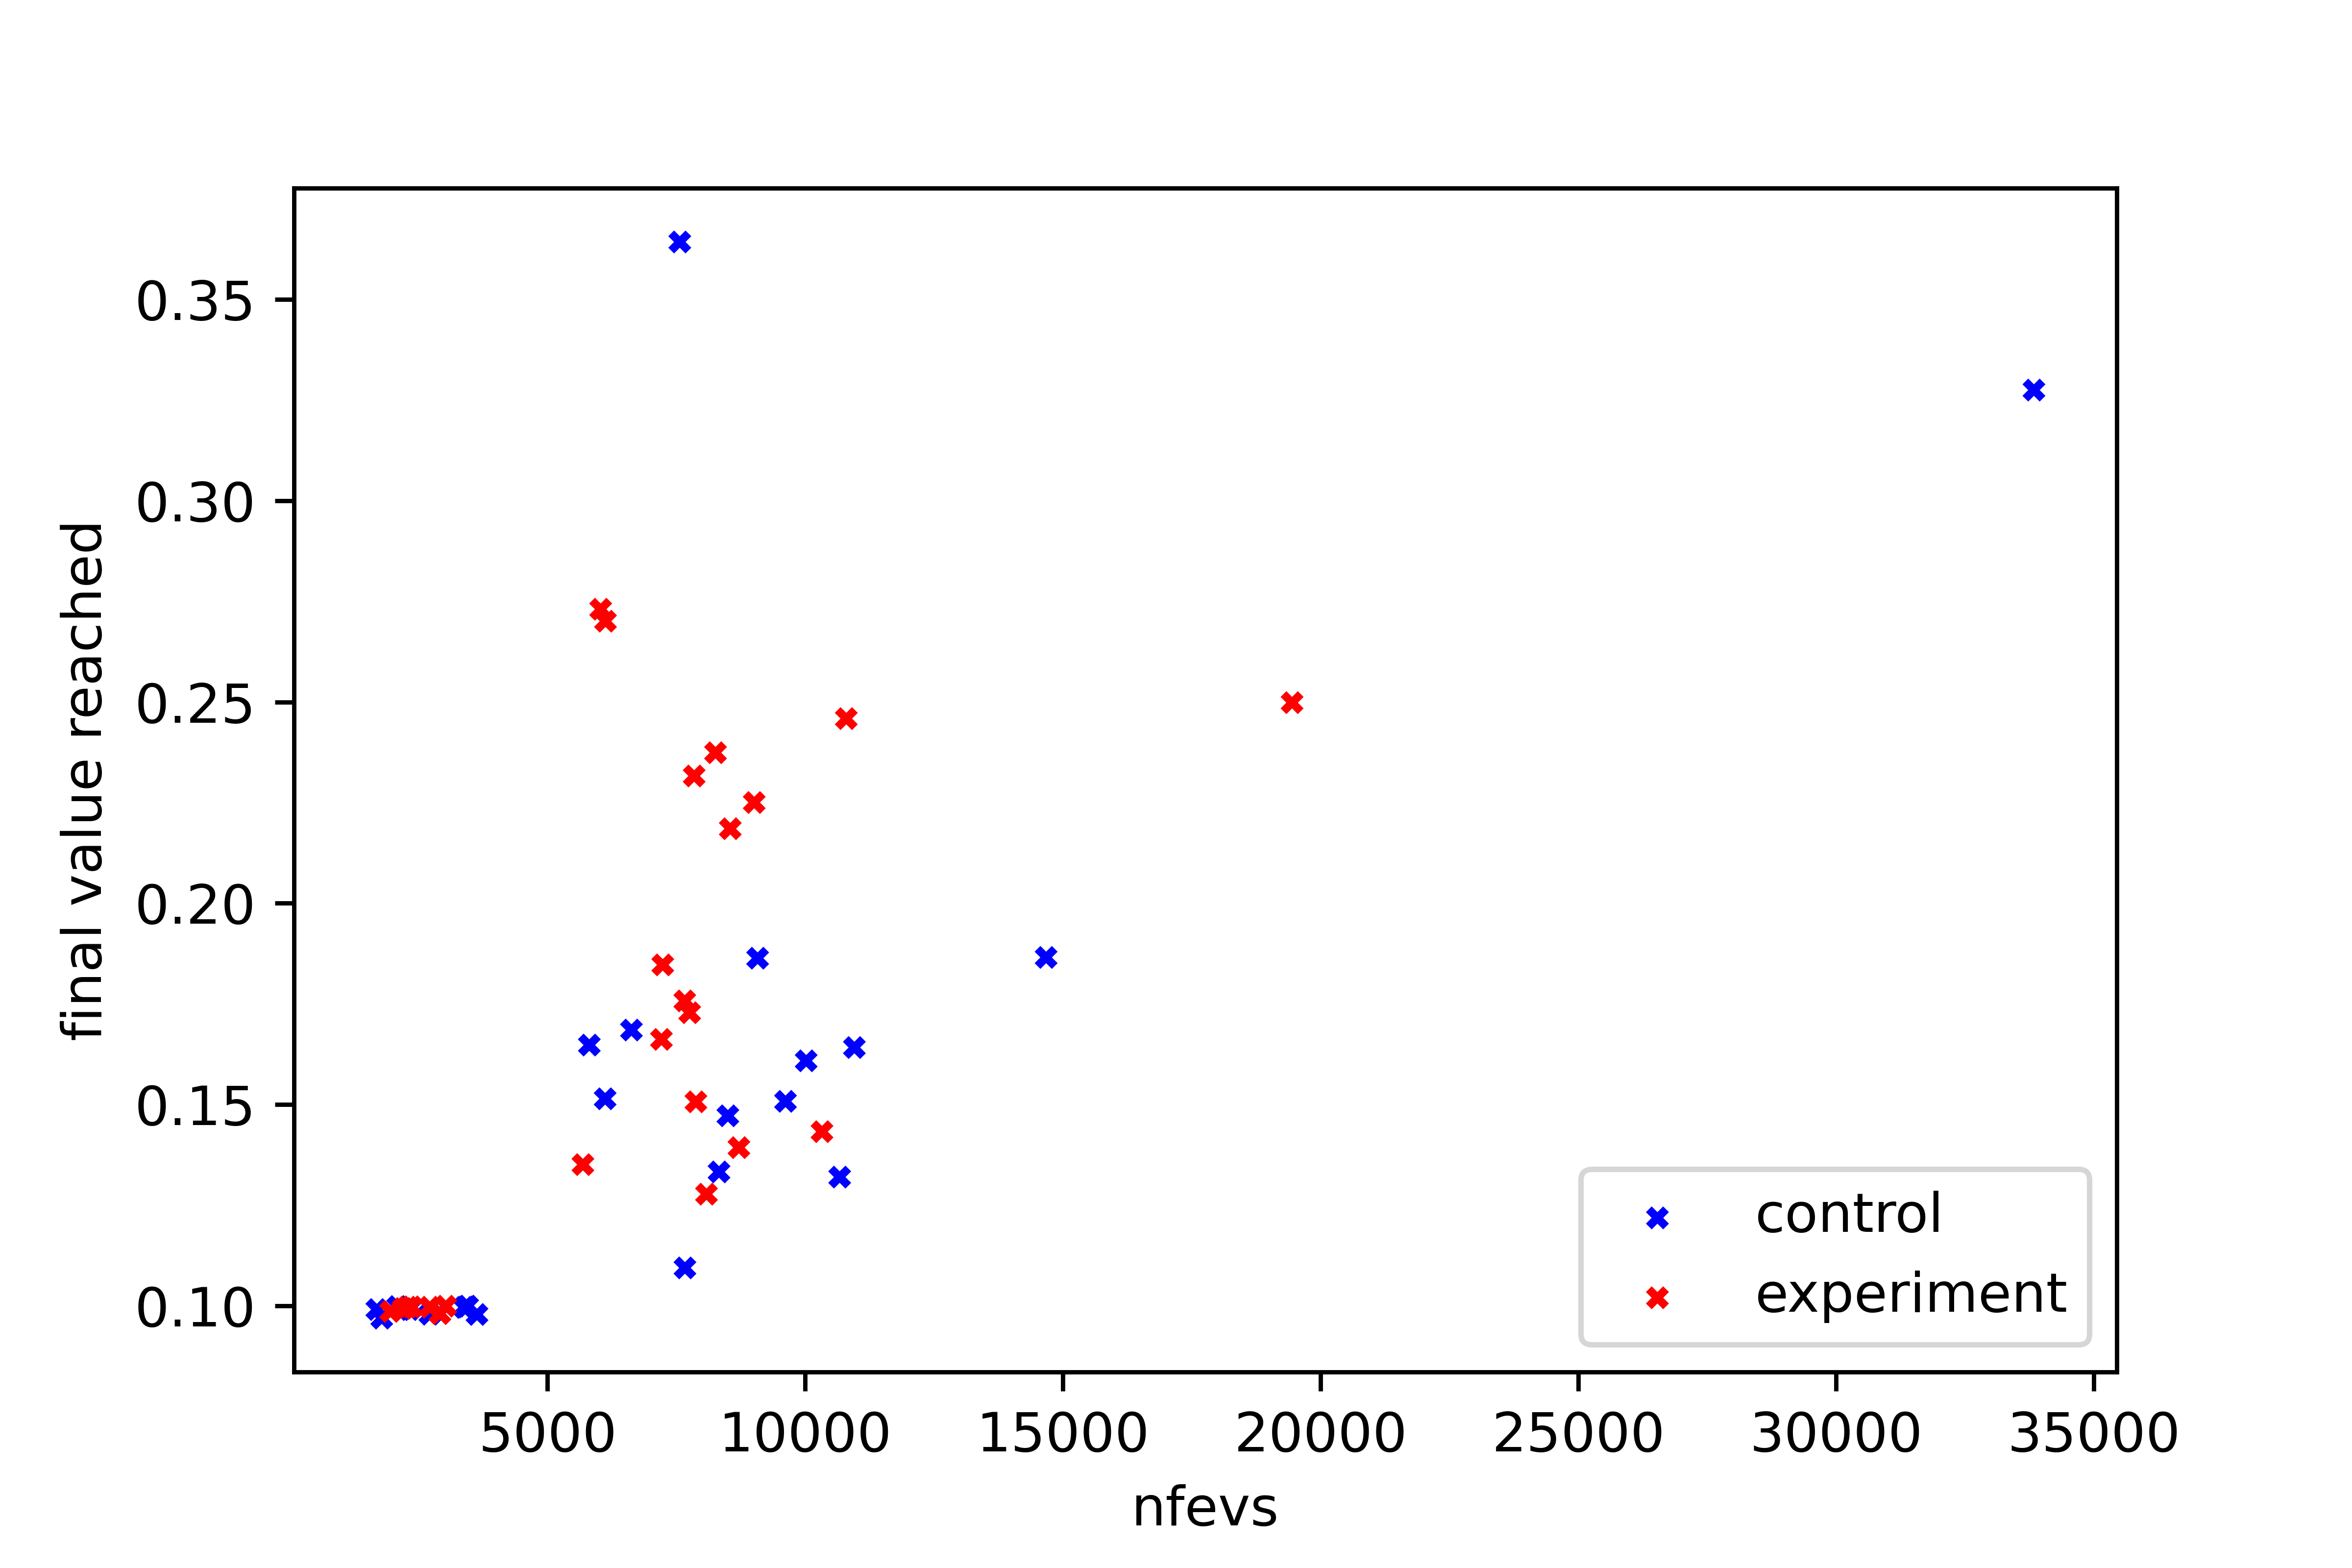
\includegraphics[scale=0.8]{7qubits.png}
    \caption{A scatter plot of the results of Experiment 2. The x-axis shows the nfevs of each experiment, and the y-axis shows the value at which the optimization halted.}
    \label{fig:7qubits}
\end{figure}

One outlier from the control group was removed, as it had more than 175000 nfevs (and, of course, failed).
As shown in the scatter plot, the control group and the Half-MUB-based experiments behaved similarly, with no clear advantage.
Although the control group had more outliers in terms of final values and nfevs, they can be dismissed as statistical anomalies.

As the plot is unclear near the $0.1$ mark, I will write out the results there: 10/25 of the control group reached $C=0.1$, and only 7/25 of the half-MUB experiments reached $C=0.1$.

Thus, my conclusion is that even with more than 3 qubits, there is no advantage to using Half-MUB states as initial states over random initial parameter vectors.

The code for the experiments in this subsection can be found in the section ``Experiment Set \#3: 7 qubits, 7 layers'' in the notebook ``bps.ipynb''.
Convergence graphs for each one of the experiments can be found in the ``VQC results/local cost 7 qubits'' subfolder. A text file with statistics and all evaluations can be found in the same folder, and used for the generation of future statistics. Details on the structure of the text file can be found in the appendix.

The same method was also implemented with 2-qubit MUB states.
The required functions for its execution are in the notebook, beside the functions for the 3-qubit MUB states.


\section{Discussion}
In this project, I have studied many different aspects of Optimization, Near-Term Quantum Computing, and Quantum Information.
Tal and I tried to apply this knowledge to try and mitigate the challenge of Barren Plateaus. Unfortunately, we did not succeed. However, I believe that this idea does not end here.
There are more experiments to be made, and there are more methods to try to fully explore this idea.
Many experimental choices were made ``Ad-Hoc'' and due to intuition --- perhaps doubling back and trying different hyper-parameter choices could lead to interesting conclusions.
I will discuss ideas for future work in the following section.

\section{Future Work}
I will now list the ideas for the continuation of this work that I could not implement myself, either due to lack of time or due to lack of specific expertise.

\paragraph*{Concentration of Measure.}
As mentioned in Section~\ref{sec:mub_use}, the Non-Uniformity of state spaces is connected to the definition of the Haar Measure and to the concentration of measure.
These subjects belong to the field of Measure Theory.
While I do not have mathematical expertise in Measure Theory, understanding the mathematical implications of these subjects on our method could be critical in two different ways: Either supply some information or constraints to our method in order to assure its advantage or show formally that it cannot give any advantage.

\paragraph*{Trying Different Hyper-Parameters.}
In Section~\ref{sec:experiments}, I made certain choices regarding hyper-parameters out of intuition or lack of time.
Examples of such choices are the values of the tolerance condition, success bound, and even the optimizer (the removal of Nelder-Mead as a candidate).
It is possible that by making these choices, I have missed some important factor.
For example, it may be that if I checked more (and higher) success bounds, a clearer distinction between MUB and non-MUB experiments could be made --- both with lower success bounds in the 3 qubit case and with higher success bounds in the 7 qubit case.

\paragraph*{Different Repetition Structure.}
While doing 25 repetitions of each experiment took a long time, it is not a parameter for completeness.
There are MUB sets with 9 MUBs for 3-qubit systems, and each one of them contains 8 states, which brings a total of 72 states.
This means, as a matter of fact, we explored around a third of all MUB states in Experiment 2.
In Experiment 3, the gap is even more apparent: there are ${7 \choose 3} = 35$ choices for triplets in 7 qubits, which brings a total of $35 \times 72 = 2520$ initial states.

Testing with much more repetitions might reveal that the results we got in Experiments 2 and 3 are no more than a statistical ``fluke'' and that our method is successful in the general case.

Another issue is that, in the cases where MUBs were used, a single initial vector was used.
This means that if it was a particularly bad choice, it could theoretically affect the whole experiment.
If our initial conjecture is correct, then this does not matter, as MUB states span the entire state space, and are only partially ``hindered'' by the initial choice.
However, a process to differentiate between the $k$ value and the number of experiment-set repetitions would not be difficult, but would definitely be beneficial.

\paragraph*{Full MUBs for Higher Qubit Counts.}
In this project, I used the examples in Lawrence~\cite{lawrence_mutually_2002} to calculate MUB sets for 2 and 3 qubits. However, there is no real reason to stop there: The work in~\cite{bandyopadhyay_new_2002} shows a construction for MUB sets for any number of qubits.
It might be the case that although Half-MUBs do not give an advantage with many qubits, and full MUB states do not give an advantage with 3 qubits, full MUB states with many qubits could provide a real advantage over random parameter choices.
Thus, putting a concentrated effort into the generation of MUB sets for $N$ qubits could be an important direction for this method.

\paragraph*{Other VQAs.}
While the Arrasmith paper~\cite{arrasmith_effect_2021} focused on the VQC problem, there is no reason to only explore this specific problem.
Other problems were explored in the context of barren plateaus, such as VQE in the original McClean paper~\cite{mcclean_barren_2018}, and the use of quantum auto-encoders in~\cite{cerezo_cost_2021}.
I tried to apply the presented ideas to VQE in this project, but the matter was left outside of scope due to time considerations. This application could have a deeper intuitive meaning, as described at the start of Section~\ref{sec:mub_use}, because the goal of the method is to reach a state (and not a transformation).
An initial sketch of how to use MUBs for Subspace VQE \cite{nakanishi_subspace-search_2019} can be found in the document ``Tal's SSVQE idea'' under the ``goals and ideas'' folder.

\paragraph*{Novel Optimization Methods.}
% Usually, the optimizers in VQAs work in the following manner:
% \begin{enumerate}
%     \item Start with a parametrized circuit (which spans the entire space), and a \emph{random} initial guess of parameters $\thetas_0$.
%     \item Run the circuit, and get an initial cost evaluation (based on$\thetas_0$).
%     \item Use an optimizer to calculate the new parameters: $\thetas_1$.
%     \item Repeat until convergence of the optimizer.
% \end{enumerate}

% Tal and I considered a different idea, which uses the cost function value at \emph{multiple, different locations} as part of this optimization. Using this kind of optimizer, we could use the following method:
% \begin{enumerate}
%     \item 	Start with a parametrized circuit (which spans the entire space), and a \emph{random} initial guess of parameters $\thetas_0$.
%     \item Run the circuit and get an initial cost evaluation (based on$\thetas_0$).
%     \item Now consider the same parametrized circuit, and a \emph{random} iniital guess of parameters $\thetas_1$.
%     \item Run the circuit and get an initial cost evaluation (based on$\thetas_1$).
%     \item Use a special optimizer, 	that takes the TWO evaluations, to calculate the new parameter: $\thetas_2$.
%     \item Repeat until convergence of the optimizer, using multiple values for $\thetas$. Either use ALL thetas (the optimizer needs to be able to work on a variable amount of cost function evaluations), or use the last/best two thetas to calculate the next one (a-la-momentum GD).
% \end{enumerate}
All of the optimizers we considered in our project worked in a relatively standard way: they consider a single point in parameter space $\thetas_i$ and use it to find the next point $\thetas_{i+1}$. An interesting idea would be to use a different kind of optimizer: One that uses \emph{multiple} points in the parameter space in order to find the next point of interest. For example, an optimizer that calculates the next step from $k$ points in the parameter space could start with all MUB states as initial points.

While multi-point optimizers exist (such as Momentum Gradient Descent), we could not find one that is fit for our idea.
Finding (or perhaps constructing) such an optimizer could use the important data that MUB states contain in a more meaningful and effective way.


More details can be found in the document ``Tal's optimization idea.docx'' under the ``goals and ideas'' subfolder.



\printbibliography

\appendix

\section{Structure of Statistics Files}
Each experiment set's results were saved in statistics files called ``stats.txt''.
These files contain a python dictionary, so they can be loaded directly into python for the generation of future statistics.

Each statistics file describes experiments with \textbf{specific} parameters and hyper-parameters.
Thus, for example, Experiment Set \#1's results are spread over several statistics files.

The statistics files contain two main types of data:
\begin{enumerate}
    \item Raw convergence data. For every experiment run, a list of all convergence values is saved.
    This list functions as a function from iteration no. to the value of the function in that iteration.
    Convergence graphs can be generated directly from this data.
    It is saved under the label `evals'.
    \item Statistical data. this is data that was generated from the raw convergence data and is usually relevant for experiments.
\end{enumerate}

The statistical data contains the following fields:
\begin{denseitemize}
    \item `avg\_nfev': The average nfev for all experiments described by the file.
    \item `correct\_addition\_percent': The fraction of iterations that managed to reach the success bound.
    \item `correct\_states' (non-control-group): The MUB or Half-MUB states that managed to reach the success bound.
    \item `correct\_states/thetas\_count': the \emph{number} of iterations that managed to reach the success bound.
    \item `fin\_vals': The values on which each experiment halted its optimization.
    \item `min\_nfev': The minimal nfev from all experiments.
    \item `nfevs': The number of function evals that each optimization experiment had until it halted.
\end{denseitemize}

\end{document}
